\documentclass[10pt]{extarticle}
\usepackage{amsmath}
\usepackage{amsfonts}
\usepackage{amssymb}
\usepackage{extsizes}
\usepackage{float}
\usepackage{graphicx}
\usepackage[margin = 1in]{geometry}
\usepackage{hyperref}
\usepackage[english]{babel}
\usepackage[backend=biber, style=numeric]{biblatex}
\usepackage[skins, minted]{tcolorbox}
\usepackage[T1]{fontenc}
\usepackage{lmodern}

\addbibresource{refs.bib}

\usepackage{minted}
\tcbset{listing engine=minted}
\tcbuselibrary{breakable}
\setminted{
	fontsize = \tiny, 
	breaklines,
	linenos = 1,
	numbersep = 2mm,
	autogobble,
	frame = none,
	style = friendly
}

\definecolor{rblue}{HTML}{75AADB}
\definecolor{stanred}{HTML}{B2001D}
\definecolor{jagsyellow}{HTML}{FFCB00}
\newtcbinputlisting{\tcbr}[1]{
	listing file = #1, 
	listing only, 
	minted language = R, 
	title = \lstinline{#1}, 
	minted options = 
	{
		fontsize = \scriptsize, 
		breaklines,
		linenos,
		numbersep = 2mm,
		frame = none,
		style = friendly,
		xleftmargin = 12pt
	}, 
	breakable,
	boxrule = 1pt,
	colback = white,
	colframe = rblue
}
\newtcbinputlisting{\tcbstan}[1]{
	listing file = #1, 
	listing only, 
	minted language = Stan, 
	title = \lstinline{#1}, 
	minted options = 
	{
		fontsize = \scriptsize, 
		breaklines,
		linenos,
		numbersep = 2mm,
		frame = none,
		style = friendly,
		xleftmargin = 12pt
	}, 
	breakable,
	boxrule = 1pt,
	colback = white,
	colframe = stanred
}
\newtcbinputlisting{\tcbjags}[1]{
	listing file = #1, 
	listing only, 
	minted language = R, 
	title = \lstinline{#1}, 
	minted options = 
	{
		fontsize = \scriptsize, 
		breaklines,
		linenos,
		numbersep = 2mm,
		frame = none,
		style = friendly,
		xleftmargin = 12pt
	}, 
	breakable,
	boxrule = 1pt,
	colback = white,
	colframe = jagsyellow
}
\usepackage{lstbayes}
%\usepackage[usenames,dvipsnames]{color}    

\newcommand{\E}{\mathbb{E}}
\newcommand{\Var}{\mathrm{Var}}
\renewcommand{\vec}[1]{\mathbf{#1}}
\newcommand{\Cov}{\mathrm{Cov}}


\begin{document}
	
\title{Bayesian Data Analysis Assignment 2}
\author{Benjamin Cox, S1621312}
\date{\vspace{-5ex}}
\maketitle

\section*{Question 1}

\begin{figure}[H]
	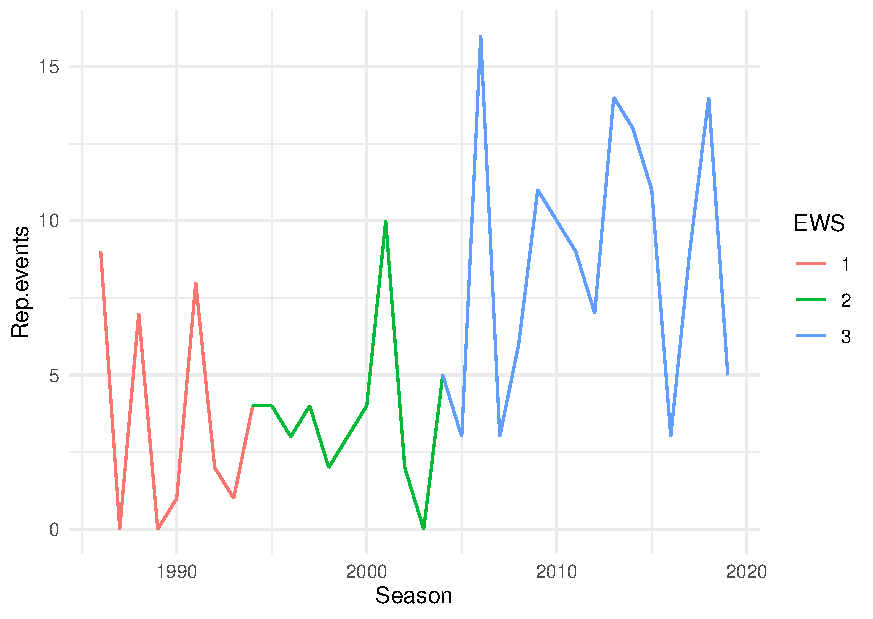
\includegraphics[width = 0.45\textwidth]{../ava_sea}
	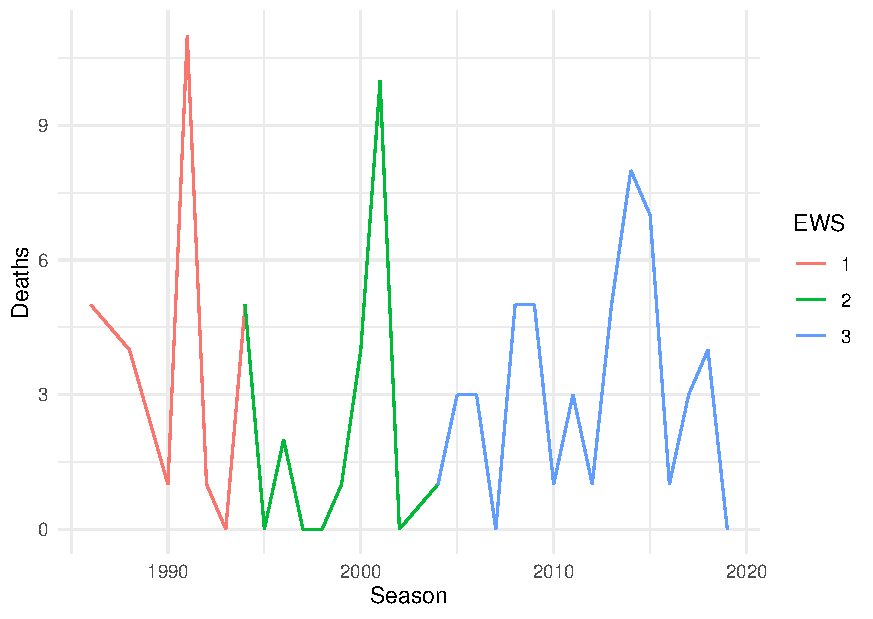
\includegraphics[width = 0.45\textwidth]{../dea_sea}
	\caption{Plots illustrating the temporal evolution of avalanche related statistics. The EWS measure is 1 = No EADS, 2 = EADS extant, 3 = EADS online daily.}
	\label{fig:tempevava}
\end{figure}	

	From the above graphs we can see a broadly positive trend in the number of avalanches and year, but no obvious trend in the number of deaths. We calculate the correlations between the number of deaths and the number of avalanches separated into EWS periods. 
	
	We obtain the following correlations (90\% bootstrap intervals)
\begin{table}[H]
	\centering
	\begin{tabular}{ccc}
		\hline
		No EADS & EADS & EADS Online \\
		\hline
		0.807 (0.6397, 0.9986) & 0.875 (0.1890, 0.9728) & 0.602 (0.3842, 0.8147) \\
		\hline
	\end{tabular}
\end{table}
This shows that the events become less correlated after the general public obtained easy access to EADS. It is not likely that the introduction of EADS increased to correlation, so the observed increase in correlation for that period is likely due to noise (10 events in 2001 resulting in 10 deaths). However it may also be due to an increase in user confidence, which led to foolish behaviour.

We are now going to model the number of deaths in avalanches. We are using a Poisson model with a logarithmic (canonical) link function. 

Our formulae are as follows:

\begin{align*}
\lambda_i &= \exp(\beta_0 + \beta_1 \cdot \mathrm{EADS1}_i + \beta_2 \cdot \mathrm{EADS2}_i + \beta_3 \cdot \mathrm{Rep.events}_i)\\
\log(\lambda_i) &= \beta_0 + \beta_1 \cdot \mathrm{EADS1}_i + \beta_2 \cdot \mathrm{EADS2}_i + \beta_3 \cdot \mathrm{Rep.events}_i\\
\mathrm{Deaths}_i &\sim \mathrm{Poisson}(\lambda_i)
\end{align*}

We could model with an offset and without a regression coefficient on the number of avalanches. That model would assume a constant rate per avalanche, which this model does not. We note that this model allows for deaths without an avalanche occurring.

We place wide normal priors on all $\beta_i$ and code up our model. The code is given in \ref{code:stan_1}, with a JAGS version given in \ref{code:jags_1}. 

We are going to run $7$ parallel chains with initial values drawn from a Uniform(-0.1, 0.1) distribution. We are going to run each chain for 3000 iterations and discard the first 1500 (HMC/NUTS converges faster than Gibbs so the length is fine). 

After running we check BGR statistics and find that they have all converged to 1. We also check NUTS specific diagnostics (divergences, energies) and find them satisfactory as well (no divergences, good energy mixing). Therefore we proceed with our analysis.

We obtain the following posterior summaries. We have exponentiated our parameters prior to summarising to ease interpretation.

\begin{table}[ht]
	\centering
\begin{tabular}{rrrrr}
	\hline
	& (Intercept) $(\beta_0)$ & Rep.events $(\beta_3)$ & EADS1TRUE $(\beta_1)$ & EADS2TRUE $(\beta_2)$\\ 
	\hline
	Min. & 0.35 & 1.09 & 0.22 & 0.12 \\ 
	1st Qu. & 0.86 & 1.19 & 0.71 & 0.32 \\ 
	Median & 1.05 & 1.22 & 0.88 & 0.39 \\ 
	Mean & 1.08 & 1.22 & 0.92 & 0.41 \\ 
	3rd Qu. & 1.26 & 1.24 & 1.08 & 0.48 \\ 
	Max. & 2.62 & 1.38 & 3.01 & 1.32 \\ 
	\hline
\end{tabular}
\caption{Posterior summaries for the first Poisson model}
\label{tab:postsum_po}
\end{table}

From this we can make some initial conclusions. We see that the expected number of deaths per year given no mitigation (ie all other covariates 0) is 1.08. We also see that each EADS evolution decreases the expected number of deaths, by 0.92 and 0.41 times respectively (if all other variables are held constant). The latter is a rather large decrease, befitting of the drastic change in preparation tact that the EADS going online brought about. We also see that each avalanche increases the number of expected deaths 1.22 times. This means that avalanches get exponentially more dangerous the more that there are, which seems somewhat strange.

We are interested in the posterior predictive distribution. We want to predict the probability of observing less than 15 deaths given 20 avalanches next year. We know that the EADS will still be online, so we have the appropriate data. 

We obtain a probability of $P(\mathrm{Deaths}<15|\mathrm{Rep.events}=20, \mathrm{EADS}=2) = 0.185$ with a 95\% bootstrap interval of $(0.1838, 0.1864)$. This is rather low, but this is expected given that large number of avalanches (and that they get more dangerous the more there are.)

We are also interested in the probability of observing more than 1 death in mean per avalanche in each stage of the EADS lifespan (not present, present, online). For this we need to calculate $$P\left(\frac{\lambda}{\mathrm{Rep.events}}>1 \ \vline \ \mathrm{EADS}=x\right).$$ Given our offsetting this is rather simple, as this simplifies to $$P\left(\exp(\beta_0 + \beta_1 \cdot \mathrm{EADS1} + \beta_2 \cdot \mathrm{EADS2}) > 1 | \mathrm{EADS} = x\right),$$
of which we have posterior samples.

We calculate these probabilities for all values of the EADS and obtain
\begin{table}[ht]
	\centering
\begin{tabular}{ccc}
	\hline
	No EADS & EADS & EADS online \\
	\hline
	0.105 & 0.005 & 0 (machine precision) \\
	\hline
\end{tabular}
\caption{Probabilities of multiple fatalities per avalanche given the various states of the EADS}
\label{tab:probmdpa}
\end{table}

After this we are told that on average the number of avalanches per year is between 5 and 15, and that they consider that for an extreme number of events that the number of casualties could be 4 times greater (or lesser) than the average number of casualties. 

From this we work out that the mean number of avalanches is 10 with standard deviation 5. We also want to give the multiplier high mass between 0.25 and 4. 

Suggested is a log-normal prior with mean 0 and standard deviation 2 on $\phi = \exp((x-\mu_x)\cdot\beta_{\mathrm{Rep.events}}),$ the multiplier. This implies a normal prior with mean 0 and standard deviation 2 for $(x-\mu_x)\cdot\beta_{\mathrm{Rep.events}}$, or $\beta_{\mathrm{Rep.events}} \sim N(\mu = 0, \sigma^2 = 4(x-\mu_x)^2).$ There could be problems with this, as it is possible for $(x-\mu_x)$ to be 0. 

The mean and standard deviation parameters for a lognormal distribution are typically given as the mean and standard deviation of the underlying normal distribution. Hence we calculate the true mean and SD as \[\mu_{\phi} = \exp\left(0 + \frac{2^2}{2}\right) = e^2 \approx 7.39, \qquad \sigma^2_{\phi} = (\exp(2^2)-1)\exp(2\cdot0 + 2^2) = e^8 - e^4 \approx 2925, \implies \sigma \approx 54.\] This is clearly not appropriate for the multiplier, as the mean is too high, and the standard deviation even moreso.

We are now going to expand our model to include a term to capture randomness not accounted for by the other components. We are going to design the model as follows

\begin{align*}
\theta_{hyp} &\sim \mathrm{Uniform}(0, 10),\\
\theta &\sim \mathrm{Normal}(0, \theta_{hyp}),\\
\lambda_i &= \exp(\beta_1 \cdot \mathrm{EADS1}_i + \beta_2 \cdot \mathrm{EADS2}_i + \beta_3 \cdot \mathrm{Rep.events}_i + \theta)\\
\log(\lambda_i) &= \beta_1 \cdot \mathrm{EADS1}_i + \beta_2 \cdot \mathrm{EADS2}_i + \beta_3 \cdot \mathrm{Rep.events}_i + \theta\\
\mathrm{Deaths}_i &\sim \mathrm{Poisson}(\lambda_i)
\end{align*} 

This model is a lot more computationally complex than the other model and requires us to make some tweaks to the sampling and model code in order to make it converge well. It runs significantly slower than the previous model, but we do get convergence. We have re-parametrised and de-centred the model so that it is mathematically equivalent, but we are dealing with standard normals and multiples thereof, rather than working with normals with variable $\sigma$. 

To make this model run well we must remove the intercept term. This is because $\theta$ and the intercept term serve the same purpose; capture the latent effect. Therefore the intercept term must be removed, as $\theta + \beta_0$ should be constant, but this does not constrain either of them, thus without removing the intercept we do not get convergence. We note that $\beta_0$ had a normal prior with mean 0, so $\theta$ should well compensate for it.

We are going to run $4$ parallel chains with initial values drawn from a Uniform(-0.05, 0.05) distribution. We are going to run each chain for 8000 iterations and discard the first 4000 (HMC/NUTS converges faster than Gibbs so the length is fine). We are going to increase the maximum tree depth to 15 (from 10) and increase the adaptation acceptance probability to 0.99 (from 0.8). These will help us to deal with the implied distributional shape given by the uniform-normal combination. It will significantly slow sampling, but this is required for convergence.

After running we check BGR statistics and find that they have all converged to 1. We also check NUTS specific diagnostics (divergences, energies) and find them satisfactory as well (no divergences, good energy mixing). Therefore we proceed with our analysis.

This is one of the few times I have seen JAGS converge better than Stan, as the NUTS sampler finds it somewhat tricky to deal with the implied distribution space given by the normal-uniform combination alongside the others. We have to run for more iterations and with a smaller stepping than we would like, so it takes significantly longer to run. A single chain of this model takes over 3 times as long as all of the chains of the previous model. Given all of this it should give us a lot better predictions right?

Well, no.

We obtain the following table for our posterior values

\begin{table}[ht]
	\centering
	\begin{tabular}{rrrrr}
		\hline
		& Rep.events $(\beta_3)$ & EADS1TRUE $(\beta_1)$ & EADS2TRUE $(\beta_2)$ & theta ($\theta$) \\ 
		\hline
		Min. & 1.09 & 0.26 & 0.12 & 0.37 \\ 
		1st Qu. & 1.19 & 0.73 & 0.32 & 0.89 \\ 
		Median & 1.22 & 0.89 & 0.40 & 1.02 \\ 
		Mean & 1.22 & 0.93 & 0.42 & 1.06 \\ 
		3rd Qu. & 1.24 & 1.08 & 0.49 & 1.21 \\ 
		Max. & 1.36 & 2.99 & 1.34 & 3.35 \\ 
		\hline
	\end{tabular}
\caption{Posterior summaries for the second Poisson model, which attempts to encapsulate the extra variability}
\label{tab:postsum_poexv}
\end{table}

Observe that these are mostly the same as the estimates that we got above, with the exception that we have $\theta$ rather than $\beta_0$. However $\theta$ has different distributional properties not captured in this table that make it somewhat better for this task. 

Now we are going to compare the two models and make some recommendations. Comparing the posterior predictives for the data they give identical results: 

\begin{figure}[H]
	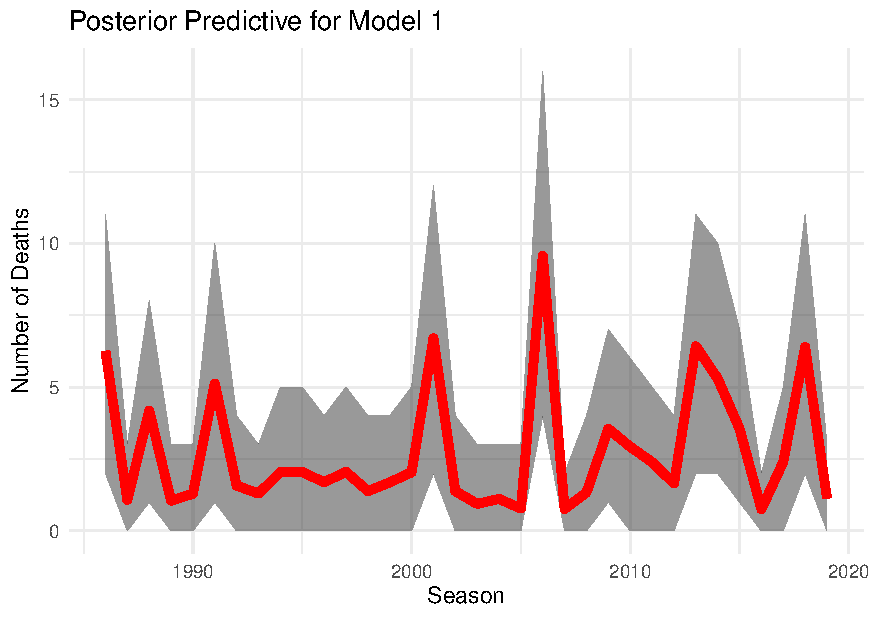
\includegraphics[width = 0.45\textwidth]{../ppmod1}
	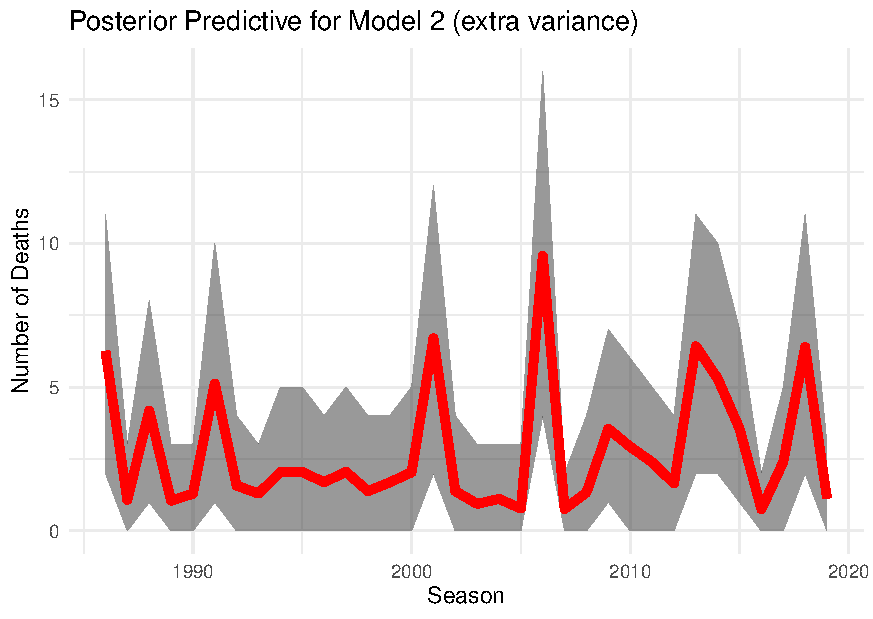
\includegraphics[width = 0.45\textwidth]{../ppmod2}
	\caption{Posterior predictive plots for the data. Note that they are identical. the red line indicates the predictive mean, and the bands indicate the 90\% credible interval.}
	\label{fig:postpreddata}
\end{figure}

Comparing the parameter summaries tells a similar story: 

\begin{figure}[H]
	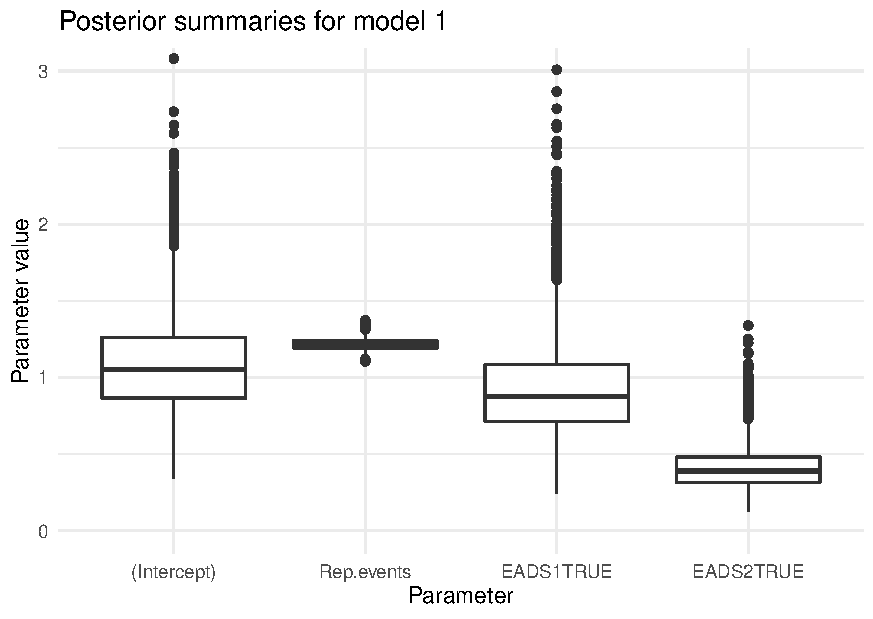
\includegraphics[width = 0.45\textwidth]{../psmod1}
	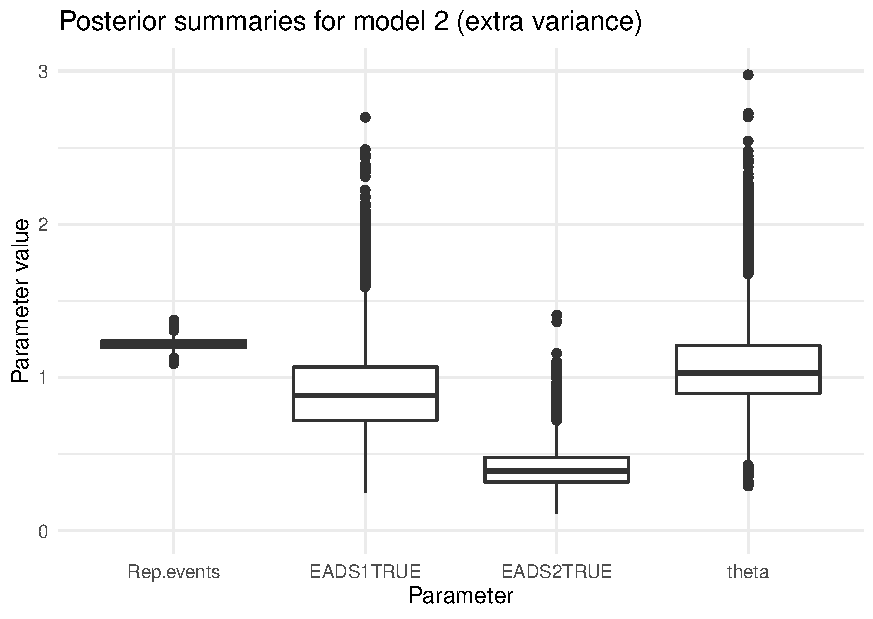
\includegraphics[width = 0.45\textwidth]{../psmod2}
	\caption{Posterior summaries for the parameters for each model. The parameters have been exponentiated to ease interpretation.}
	\label{fig:postsummods}
\end{figure}
We see that there is more variability in theta than in the intercept, but both models will lead to the same conclusions as they are very similar in terms of distribution. 

Calculating the Deviance Information Criterion for both models we get a DIC of 141.9 for the first model and a DIC of 141.6 for the second. Based on this we would weakly prefer the second model, as it has a smaller DIC. 

However I would prefer the first model. The DICs are very similar in size, and given the stochastic nature overlap distributionally quite a bit. However the first model is both more interpretable and more stable. The first model converges better and samples faster. Both lead to the same conclusions, so I don't see much reason to choose the second. 

However I propose a third model. I believe that a model of the first form with the number of avalanches as an offset rather than as a covariate makes the most sense. This is because it would mean that each avalanche is not inherently more dangerous than the last. It would also ease interpretation further, as the calculated rates would be deaths per avalanche. Furthermore it would eliminate the predictions of deaths without avalanches occurring, which is a problem with the two previous models. 

However it would not account for some years having more avalanches and thus being more dangerous than other years. I believe that this model makes more sense (and believed that it was the model we were being asked to work on prior to corresponding with the lecturer), but the biggest weakness is what I just mentioned. This model is more classical Poisson, but does not allow for some more advanced deductions. 

\section*{Question 2}

\printbibliography

\newpage

\appendix

\section{Code for Question 1}
\subsection{R}
%\inputminted{R}{../Q1.R}
\tcbr{../Q1.R}
\label{code:main_1}
\subsection{Stan}
\tcbstan{../stan/poisson_glm.stan}
\tcbstan{../stan/poisson_glm_exvar.stan}
\label{code:stan_1}
\subsection{JAGS}
\tcbr{../jags/Q1jags.R}
\tcbjags{../jags/poisson.jags}
\tcbjags{../jags/poisson_exvar.jags}
\label{code:jags_1}
\section{Code for Question 2}
\subsection{R}
\tcbr{../Q2.R}
\label{code:main_2}
\subsection{Stan}
\tcbstan{../stan/binomial_glm.stan}
\tcbstan{../stan/binomial_glm_randomeffects.stan}
\label{code:stan_2}
\end{document}

